\chapter{系统实现、测试与性能分析}

系统架构设计、核心算法研究等完成之后,就是系统的实现阶段,这是一个从理论到实践的过程,也是极具挑战的一个过程,系统不仅需要完善的功能,还需要满足性能、安全、好用的不同需求,经过几个月的研发测试,最终完成了功能完善、性能优秀的战术数据链信息标准数据库系统。

\section{系统实现架构}

\subsection{整体实现架构}

基于微服务架构的分布式架构设计理念是将系统架构作为基础设计模式,通过这种基础设计模式提供的服务间松耦合、独立部署、弹性伸缩的灵活扩展能力,便于系统的维护与扩展。微服务架构将一个复杂的应用程序系统拆分为多个相对独立的服务,每个服务负责特定的业务领域,每个服务将关注点分离、业务逻辑独立。

系统构建了9大微服务,每个微服务都有其明确的职责界限,每个微服务都有独立的控制其生命周期,每个微服务都可以进行开发、测试、部署和扩展,从而提高开发效率和灵活性。每个微服务都必须遵循单一直责任原则,保证微服务内的高内聚,并且通过统一的RESTful API接口进行微服务间的低耦合。

数据存储架构以MySQL8.0为主数据库、以Redis分布式缓存数据库为辅数据库,之所以选择MySQL,原因在于其具备高事务、支持外键约束、支持全文索引等能力,可以满足数据一致性需求,而之所以选择Redis分布式缓存数据库,原因在于其具备高查询性能与速度。

在技术栈的选型方面,选用最新技术组合,python3.10 + FastAPI + React18 + MySQL8.0+Redis。FastAPI为微服务的基石,其主要功能有高性能异步处理、自动生成API文档、类型安全等。React18作为前端应用通过RESTful API与后端微服务进行对接,前后端分离。

容器化部署作为微服务架构的重要支撑技术,系统采用Docker容器化技术将每个微服务构建成单独的容器镜像,通过 Kubernetes 对这些容器进行编排管理,这种部署架构能够提供快速部署、自动扩容、自动恢复等技术能力,能够为系统的运维管理提供良好的技术保障。

\section{微服务架构实现}

基于第四章的微服务架构设计,本节重点阐述系统的具体实现方案,包括微服务部署与通信、数据管理与存储、监控与容错三个核心方面。

\subsection{微服务部署与通信}

微服务的构建先解决服务的部署问题和通信问题,部署问题:采用 Docker 容器化部署服务,每一个微服务就是一个 Docker 容器,保证部署环境一致和部署可重用性。采用 Kubernetes 集群作为 Docker 容器的编排工具,对服务进行调度、扩缩容、生命周期管理。以声明方式部署和维护服务。

服务间通信方面,构建了同步和异步两种通信机制,其中,同步通信基于HTTP协议,服务之间使用REST API通信协议,支持JSON格式数据交换和标准HTTP状态码处理;异步通信则支持了发布/订阅和Point对点通信模式,将RabbitMQ用于异步消息队列方式,实现了服务之间消息解耦以及消息传递的效果。

微服务的部署以及服务间通信的整体部署架构如图\ref{fig:microservice_deployment}所示,包含Docker容器化部署、Kubernetes微服务集群、服务通信架构。

\begin{figure}[H]
    \centering
    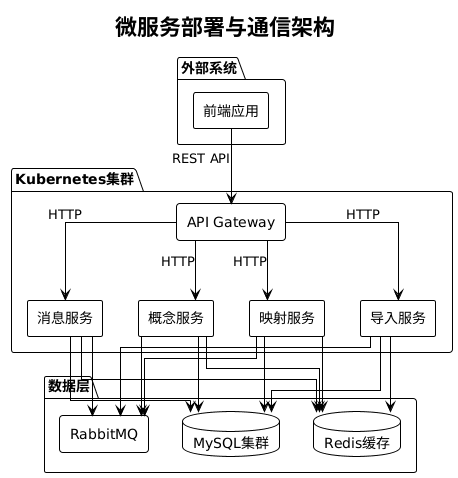
\includegraphics[width=0.8\textwidth]{chapters/fig-0/microservice_deployment.png}
    \caption{微服务部署与通信架构图}
    \label{fig:microservice_deployment}
\end{figure}

\subsection{数据管理与存储}

分布式数据存储是微服务架构系统中的关键。通过数据库分片,将数据分片存储,每个微服务负责管理一个数据片,每个数据片通过微服务进行分布式存储访问。而选择主从复制机制,通过将写操作操作到主库中,读操作则分散至多个从库中,从而实现高并发访问。

缓存采用 Redis 缓存系统,实现高速的缓存服务。采用多级缓存架构:应用缓存、分布式缓存、CDN 缓存。采用缓存预热、更新、失效策略保证缓存数据的一致性和有效性。

图\ref{fig:data_management}展示了分布式数据管理与存储架构,包括数据库分片、读写分离和缓存系统。

\begin{figure}[H]
    \centering
    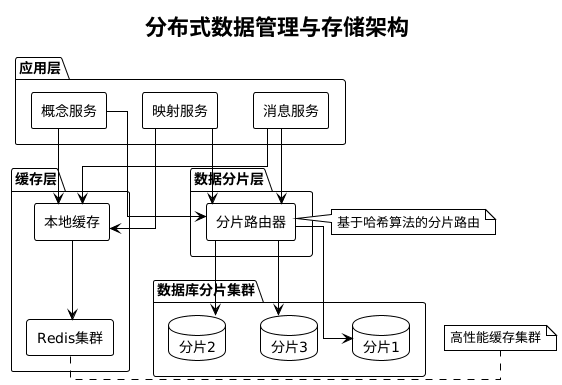
\includegraphics[width=0.8\textwidth]{chapters/fig-0/data_management.png}
    \caption{分布式数据管理与存储架构图}
    \label{fig:data_management}
\end{figure}

数据分片算法的核心实现如下:

\begin{algorithm}[H]
\caption{数据分片算法}
\begin{algorithmic}[1]
\REQUIRE data: 待分片的数据, shard\_key: 分片键, num\_shards: 分片数量
\ENSURE shard\_id: 分片ID
\STATE 计算分片ID
\STATE hash\_value $\leftarrow$ hash(shard\_key)
\STATE shard\_id $\leftarrow$ hash\_value mod num\_shards
\STATE 获取分片数据库连接
\STATE shard\_config $\leftarrow$ SHARD\_CONFIGS[shard\_id]
\STATE shard\_db $\leftarrow$ connect\_database(shard\_config)
\STATE 存储数据到对应分片
\STATE shard\_db.insert(data)
\RETURN shard\_id
\end{algorithmic}
\end{algorithm}

\subsection{监控与容错}

服务监控体系是微服务系统能否正常工作的基础,系统集成Prometheus软件系统集成为指标收集平台,通过自定义指标以及系统指标监控服务状态和性能。Grafana是可视化监控平台,提供图表、表板实时监控和历史分析功能。

容错机制通过熔断器模式和重试模式来实现。熔断器模式,服务调用失败达到预设次数时自动触发熔断模式,防止连锁故障。重试模式,使用指数退避算法对临时性故障进行智能重试,提高可靠性。

图\ref{fig:monitoring_fault_tolerance}展示了监控与容错系统的整体架构,包括Prometheus指标收集、Grafana可视化监控和熔断器容错机制。

\begin{figure}[H]
    \centering
    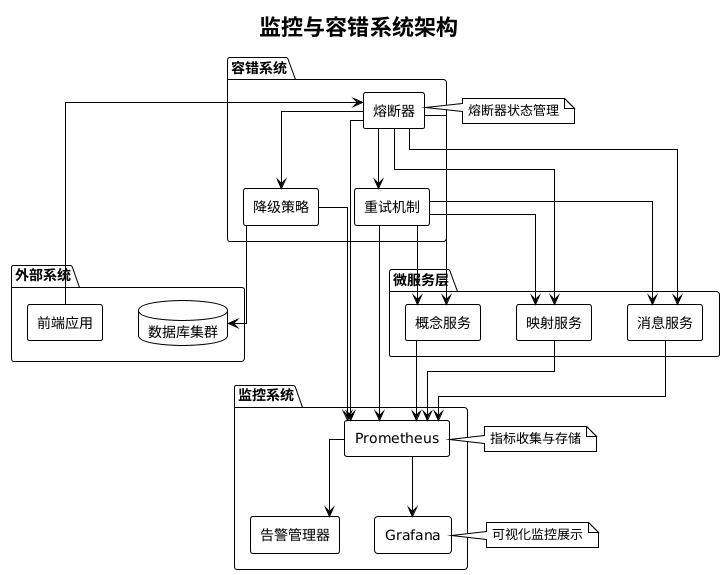
\includegraphics[width=0.8\textwidth]{chapters/fig-0/monitoring_fault_tolerance.png}
    \caption{监控与容错系统架构图}
    \label{fig:monitoring_fault_tolerance}
\end{figure}

熔断器模式的核心实现如下:

\begin{algorithm}[H]
\caption{熔断器模式算法}
\begin{algorithmic}[1]
\REQUIRE func: 待调用函数, failure\_threshold: 失败阈值, timeout: 超时时间
\ENSURE result: 函数执行结果
\STATE 初始化熔断器状态
\STATE failure\_count $\leftarrow$ 0
\STATE last\_failure\_time $\leftarrow$ null
\STATE state $\leftarrow$ 'CLOSED'
\IF{state = 'OPEN'}
    \IF{current\_time - last\_failure\_time > timeout}
        \STATE state $\leftarrow$ 'HALF\_OPEN'
    \ELSE
        \STATE 抛出异常 CircuitBreakerOpenException
    \ENDIF
\ENDIF
\STATE 尝试执行函数
\STATE 执行函数调用
\STATE result $\leftarrow$ func(*args, **kwargs)
\IF{执行成功}
    \STATE on\_success()
    \RETURN result
\ELSE
    \STATE on\_failure()
    \STATE 抛出异常 e
\ENDIF
\end{algorithmic}
\end{algorithm}

\begin{algorithm}[H]
\caption{熔断器成功处理}
\begin{algorithmic}[1]
\STATE failure\_count $\leftarrow$ 0
\STATE state $\leftarrow$ 'CLOSED'
\end{algorithmic}
\end{algorithm}

\begin{algorithm}[H]
\caption{熔断器失败处理}
\begin{algorithmic}[1]
\STATE failure\_count $\leftarrow$ failure\_count + 1
\STATE last\_failure\_time $\leftarrow$ current\_time
\IF{failure\_count >= failure\_threshold}
    \STATE state $\leftarrow$ 'OPEN'
\ENDIF
\end{algorithmic}
\end{algorithm}

表\ref{table:monitoring_metrics}列出了系统监控的关键指标和阈值配置。

\begin{table}[H]
    \caption{系统监控关键指标配置}
    \label{table:monitoring_metrics}
    \centering
    \begin{tabular}{llll}
        \toprule
        \textbf{指标类型} & \textbf{指标名称} & \textbf{阈值} & \textbf{告警级别} \\
        \midrule
        性能指标 & 响应时间 & >2秒 & 警告 \\
        性能指标 & 吞吐量 & <100 req/s & 警告 \\
        可用性指标 & 服务可用率 & <99.9\% & 严重 \\
        可用性指标 & 错误率 & >5\% & 严重 \\
        资源指标 & CPU使用率 & >80\% & 警告 \\
        资源指标 & 内存使用率 & >85\% & 警告 \\
        资源指标 & 磁盘使用率 & >90\% & 严重 \\
        \bottomrule
    \end{tabular}
\end{table}

\section{数据模型实现}

数据模型实现作为系统架构的核心基础,通过精心设计的数据库表结构、高效的索引策略和完善的约束机制,为战术数据链信息标准数据库提供了坚实的数据存储与管理基础。本节将从数据库表结构设计、索引策略优化、约束机制保障以及版本管理四个维度详细阐述数据模型的实现方案。

\subsection{数据库表结构设计}

数据库表结构设计构成了系统数据模型的基础架构。系统设计了MESSAGE、STDVERSION、FIELD、CONCEPT、MAPPING等核心数据表,这些表通过外键关联形成了完整的关系型数据模型。每个表都具有明确的职责分工,表之间的关系设计清晰合理,充分体现了第三范式(3NF)的设计原则。

以下SQL代码定义了核心数据表结构,该实现包括主外键约束、索引策略和数据完整性检查:

\begin{algorithm}[H]
\caption{数据库表结构设计}
\begin{algorithmic}[1]
\REQUIRE 表结构需求 \\
\ENSURE 完整的数据库表结构 \\
\STATE 创建标准版本表
\STATE CREATE TABLE STD\_VERSION
\STATE std\_id: VARCHAR(36) PRIMARY KEY
\STATE std\_name: VARCHAR(64) NOT NULL
\STATE version\_number: VARCHAR(32) NOT NULL
\STATE 创建消息表
\STATE CREATE TABLE MESSAGE
\STATE message\_id: VARCHAR(36) PRIMARY KEY
\STATE j\_num: VARCHAR(16) NOT NULL
\STATE title: VARCHAR(128) NOT NULL
\STATE std\_id: VARCHAR(36) NOT NULL
\STATE FOREIGN KEY (std\_id) REFERENCES STD\_VERSION(std\_id)
\STATE 创建字段表
\STATE CREATE TABLE FIELD
\STATE field\_id: VARCHAR(36) PRIMARY KEY
\STATE message\_id: VARCHAR(36) NOT NULL
\STATE start\_bit: INT NOT NULL
\STATE end\_bit: INT NOT NULL
\STATE FOREIGN KEY (message\_id) REFERENCES MESSAGE(message\_id)
\end{algorithmic}
\end{algorithm}

\subsection{索引策略优化}

索引策略的实现对系统查询性能具有至关重要的影响。系统实现了组合索引、覆盖索引以及全文索引等多种索引类型,通过合理的索引设计显著提升了数据库的查询效率。组合索引可以实现跨字段复合检索,组合索引避免了无意义的回表,全文索引为全文文本检索功能提供技术支持。

索引策略的核心代码如下,该实现创建了高效的查询索引,包括组合索引、覆盖索引和全文索引:

\begin{algorithm}[H]
\caption{数据库索引策略}
\begin{algorithmic}[1]
\REQUIRE 表结构和查询需求
\ENSURE 优化的索引结构
\STATE 创建字段范围索引
\STATE CREATE INDEX IDX\_FIELD\_MSG\_RANGE ON FIELD(message\_id, start\_bit, end\_bit)
\STATE 创建消息查找索引
\STATE CREATE INDEX IDX\_MSG\_LOOKUP ON MESSAGE(std\_id, j\_num)
\STATE 创建标准版本名称索引
\STATE CREATE INDEX IDX\_STD\_VERSION\_NAME ON STD\_VERSION(std\_name, version\_number)
\end{algorithmic}
\end{algorithm}

\subsection{约束机制保障}

约束的机制可以保证数据完整、数据一致性、是数据模型可靠性有效保证。系统提供了主外键约束、检查约束、触发器机制等方法等约束机制。主外键约束保证数据引用完整性、检查约束保证数据有效性、业务规则正确性、触发器机制保证复杂业务、逻辑、数据一致性的有效性。

约束机制的关键SQL代码如下,该实现定义了完整的数据完整性约束,包括主外键约束、检查约束和触发器:

\begin{algorithm}[H]
\caption{数据库约束机制}
\begin{algorithmic}[1]
\REQUIRE 表结构和业务规则
\ENSURE 完整的约束体系
\STATE 添加消息表外键约束
\STATE ALTER TABLE MESSAGE
\STATE ADD CONSTRAINT FK\_MESSAGE\_STD\_VERSION
\STATE FOREIGN KEY (std\_id) REFERENCES STD\_VERSION(std\_id)
\STATE 添加字段表外键约束
\STATE ALTER TABLE FIELD
\STATE ADD CONSTRAINT FK\_FIELD\_MESSAGE
\STATE FOREIGN KEY (message\_id) REFERENCES MESSAGE(message\_id)
\STATE 添加字段位范围检查约束
\STATE ALTER TABLE FIELD
\STATE ADD CONSTRAINT CHK\_FIELD\_BIT\_RANGE
\STATE CHECK (start\_bit >= 0 AND end\_bit > start\_bit)
\end{algorithmic}
\end{algorithm}
\subsection{版本管理}
版本管理功能是数据模型功能之一,它能够使得系统记录下标准的变化轨迹。标准版本控制、变化历史追溯、审计日志等,是系统标准版本控制的方式和工具,它为研究分析标准的变化过程、数据分析、系统维护等,提供历史数据。

版本管理功能的SQL代码实现如下,该实现提供了完整的版本控制和审计功能:

\begin{algorithm}[H]
\caption{版本管理表结构}
\begin{algorithmic}[1]
\REQUIRE 版本管理需求
\ENSURE 版本控制和审计表结构
\STATE 创建版本历史表
\STATE CREATE TABLE VERSION\_HISTORY
\STATE history\_id: VARCHAR(36) PRIMARY KEY
\STATE table\_name: VARCHAR(64) NOT NULL
\STATE record\_id: VARCHAR(36) NOT NULL
\STATE operation\_type: ENUM('INSERT', 'UPDATE', 'DELETE') NOT NULL
\STATE changed\_at: TIMESTAMP DEFAULT CURRENT\_TIMESTAMP
\STATE 创建审计日志表
\STATE CREATE TABLE AUDIT\_LOG
\STATE log\_id: VARCHAR(36) PRIMARY KEY
\STATE action: VARCHAR(100) NOT NULL
\STATE resource\_type: VARCHAR(64)
\STATE resource\_id: VARCHAR(36)
\STATE created\_at: TIMESTAMP DEFAULT CURRENT\_TIMESTAMP
\end{algorithmic}
\end{algorithm}



\section{核心功能模块实现}

系统完成了4大模块的实现,各功能模块各司其职、互相协作。4大模块通过统一接口完成交流,组成了一个完整的流水线。

\subsection{PDF处理模块实现}

PDF处理模块作为系统的重要组成部分,集成了PyMuPDF、pdfplumber、Camelot以及Tesseract OCR等多个先进工具,实现了从PDF文档中提取结构化数据的关键功能。该模块能够将多种格式的PDF文件快速解析成对应的表格、文字、图片等内容,为后续的数据处理与分析奠定基础。

以下核心代码展示了PDF处理器的关键实现,该类封装了完整的PDF文档处理流程,包括表格提取、章节解析、数据标准化和校验等功能:

\begin{algorithm}[H]
\caption{PDF处理器算法}
\begin{algorithmic}[1]
\REQUIRE pdf\_path: PDF文件路径, standard: 标准类型
\ENSURE result: 包含表格和章节的字典
\STATE 初始化PDF处理器
\STATE standard $\leftarrow$ "MIL-STD-6016"
\STATE table\_extractor $\leftarrow$ TableExtractor()
\STATE section\_parser $\leftarrow$ SectionParser()
\STATE 处理PDF文件
\STATE tables $\leftarrow$ table\_extractor.extract\_tables(pdf\_path)
\STATE sections $\leftarrow$ section\_parser.parse\_sections(pdf\_path)
\STATE 构建结果字典
\STATE result $\leftarrow$ \{"tables": tables, "sections": sections\}
\RETURN result
\end{algorithmic}
\end{algorithm}

\subsection{语义互操作模块实现}

语义互操作模块主要提供了消息语义分析、跨协议转化、语义字段标注等功能,该模块核心在于对不同协议间进行了解映射,系统的核心是采用机器学习的方法,从而对语义的相似度进行判别,提高映射的可靠性与准确性。

语义互操作管理器的核心代码如下,该管理器负责分析消息语义、执行跨协议转换和消息路由:

\begin{algorithm}[H]
\caption{语义互操作管理器算法}
\begin{algorithmic}[1]
\REQUIRE message: 消息字典, standard: 标准类型
\ENSURE semantic\_analysis: 语义分析结果
\STATE 初始化互操作性管理器
\STATE registry $\leftarrow$ SemanticRegistry()
\STATE transformer $\leftarrow$ SemanticTransformer()
\STATE 分析消息语义
\STATE message\_type $\leftarrow$ message.get("message\_type")
\STATE semantic\_fields $\leftarrow$ \{\}
\STATE 构建语义分析结果
\STATE semantic\_analysis $\leftarrow$ \{
\STATE     "message\_type": message\_type,
\STATE     "standard": standard,
\STATE     "semantic\_fields": semantic\_fields
\STATE \}
\RETURN semantic\_analysis
\end{algorithmic}
\end{algorithm}

\subsection{CDM四层法模块实现}

CDM四层法模块按语义层、映射层、校验层、运行层分层设计,语义层定义概念和理解概念,映射层映射不同协议,校验层是映射校验层,运行层是运算执行层,这种分层方式便于系统扩展、易于维护。

CDM四层法系统的关键代码片段如下,该系统按照语义层、映射层、校验层和运行层的架构实现消息转换:

\begin{algorithm}[H]
\caption{CDM互操作系统算法}
\begin{algorithmic}[1]
\REQUIRE source\_message: 源消息, source\_protocol: 源协议, target\_protocol: 目标协议
\ENSURE target\_message: 转换后的目标消息
\STATE 初始化CDM互操作系统
\STATE cdm\_registry $\leftarrow$ CDMRegistry()
\STATE converter $\leftarrow$ MessageConverter()
\STATE 处理消息转换
\STATE target\_message $\leftarrow$ converter.convert\_message(
\STATE     source\_message, source\_protocol, target\_protocol
\STATE )
\RETURN target\_message
\end{algorithmic}
\end{algorithm}

\subsection{统一导入模块实现}

统一导入模块能够导入各种文件格式,比如:PDF、XML、TXT、CSV等,软件能够自动识别并按照文件内容采取合适的方法处理。批量导入能够让用户一次录入多个不同格式文件,大大提高了工作效率。

统一导入系统的核心代码如下,该系统支持多种文件格式的自动检测和处理,提供统一的导入接口:

\begin{algorithm}[H]
\caption{统一导入系统算法}
\begin{algorithmic}[1]
\REQUIRE file\_path: 文件路径
\ENSURE result: 导入结果
\STATE 初始化统一导入系统
\STATE adapters $\leftarrow$ [PDFAdapter(), XMLAdapter(), JSONAdapter()]
\STATE 处理单个文件
\STATE format\_info $\leftarrow$ detect\_file\_format(file\_path)
\STATE adapter $\leftarrow$ select\_adapter(format\_info)
\STATE result $\leftarrow$ adapter.import\_file(file\_path)
\RETURN result
\end{algorithmic}
\end{algorithm}

此四个模块之间通过一个公共接口互相通信,构成了一个完整的处理链,每个模块各司其职,模块之间以标准化的数据类型互相通信,易于维护和扩展。




\section{后端服务实现}

\subsection{FastAPI服务架构实现}

后端服务是系统的核心,系统选择了FastAPI作为Web框架。FastAPI提供了Web服务异步、自动生成文档等诸多接口,能够极大提高开发效率。

FastAPI应用的主入口代码如下,该实现配置了完整的应用设置,包括中间件、路由注册和异常处理:

\begin{algorithm}[H]
\caption{FastAPI应用初始化算法}
\begin{algorithmic}[1]
\REQUIRE 应用配置参数
\ENSURE 配置完成的FastAPI应用
\STATE 导入FastAPI模块
\STATE from fastapi import FastAPI
\STATE from fastapi.middleware.cors import CORSMiddleware
\STATE 创建FastAPI应用实例
\STATE app $\leftarrow$ FastAPI(title="MIL-STD-6016 数据链标准系统")
\STATE 配置CORS中间件
\STATE app.add\_middleware(
\STATE     CORSMiddleware,
\STATE     allow\_origins=["*"],
\STATE     allow\_methods=["*"],
\STATE     allow\_headers=["*"]
\STATE )
\end{algorithmic}
\end{algorithm}

路由层的实现是通过 API 对各个 API 站点进行组织。路由器中每个路由都有自己的参数校验规则,确保输入数据的有效性,中间件功能包括跨域处理、请求记录、异常处理等。

路由配置的核心代码如下,该实现定义了完整的API路由结构,包括参数验证和响应模型:

\begin{algorithm}[H]
\caption{FastAPI路由配置算法}
\begin{algorithmic}[1]
\REQUIRE 路由配置需求
\ENSURE 配置完成的API路由
\STATE 导入路由模块
\STATE from fastapi import APIRouter
\STATE from pydantic import BaseModel
\STATE 创建API路由器
\STATE router $\leftarrow$ APIRouter(prefix="/api")
\STATE 定义请求模型
\STATE class SearchRequest(BaseModel):
\STATE     keyword: str
\STATE     limit: int = 100
\STATE 注册搜索路由
\STATE @router.post("/search")
\STATE async def search\_messages(request: SearchRequest):
\STATE     \RETURN \{"results": [], "total": 0\}
\end{algorithmic}
\end{algorithm}

服务层封装了业务逻辑。系统使用了注入注入的设计,使系统间的依赖更加清晰明了。系统使用了异常处理机制,使得系统在遇到错误时能够优雅的处理,不影响用户体验。

服务层的关键代码如下,该实现封装了核心业务逻辑,包括数据查询、处理和转换:

\begin{algorithm}[H]
\caption{FastAPI服务层算法}
\begin{algorithmic}[1]
\REQUIRE keyword: 搜索关键词, db: 数据库会话
\ENSURE results: 搜索结果列表
\STATE 导入异步数据库模块
\STATE from sqlalchemy.ext.asyncio import AsyncSession
\STATE 定义搜索服务类
\STATE class SearchService:
\STATE     初始化服务
\STATE     def \_\_init\_\_(self, db: AsyncSession):
\STATE         self.db $\leftarrow$ db
\STATE     执行搜索逻辑
\STATE     async def search\_messages(self, keyword: str) returns list:
\STATE         \RETURN []
\end{algorithmic}
\end{algorithm}

数据访问层基于SQLAlchemy ORM构建。系统使用了异步会话管理,提高了数据库操作的效率。连接池管理确保系统在高并发情况下能够稳定运行。

数据库连接管理的核心代码如下,该实现提供了异步数据库会话管理和连接池配置:

\begin{algorithm}[H]
\caption{数据库连接管理算法}
\begin{algorithmic}[1]
\REQUIRE 数据库连接配置
\ENSURE 配置完成的数据库连接
\STATE 导入SQLAlchemy异步模块
\STATE from sqlalchemy.ext.asyncio import create\_async\_engine, AsyncSession
\STATE from sqlalchemy.orm import sessionmaker
\STATE 创建异步数据库引擎
\STATE engine $\leftarrow$ create\_async\_engine("sqlite+aiosqlite:///./app.db")
\STATE 创建异步会话工厂
\STATE AsyncSessionLocal $\leftarrow$ sessionmaker(
\STATE     engine, class\_=AsyncSession, expire\_on\_commit=False
\STATE )
\end{algorithmic}
\end{algorithm}

API接口设计遵循RESTful规范。系统为每个资源都提供了标准的CRUD操作接口。自动文档生成功能让前端开发人员能够快速了解接口的使用方法。



\subsection{核心API接口实现}

搜索接口是系统最重要的功能之一。系统实现了/api/search接口,支持关键词搜索、J系列筛选以及模糊匹配。这个接口能够根据用户输入快速返回相关的消息字段信息。

以下是搜索接口的主要实现,该接口支持多条件搜索和分页查询,提供灵活的搜索功能:

\begin{algorithm}[H]
\caption{搜索API接口算法}
\begin{algorithmic}[1]
\REQUIRE request: 搜索请求对象
\ENSURE response: 搜索结果响应
\STATE 注册搜索路由
\STATE @router.post("/search")
\STATE 定义搜索函数
\STATE async def search\_messages(request: SearchRequest):
\STATE     执行搜索逻辑
\STATE     results $\leftarrow$ []
\STATE     total $\leftarrow$ 0
\STATE     \RETURN \{"results": results, "total": total\}
\end{algorithmic}
\end{algorithm}

比较接口/api/compare提供了跨标准版本的概念比较的标准接口。它提供了不同版本的标准之间的差异比较,并显示比较结果。聚合比较功能也允许了标准更全面地比较标准的变化。

比较接口的具体实现如下,该接口支持跨版本标准的概念比较和差异分析:

\begin{algorithm}[H]
\caption{比较API接口算法}
\begin{algorithmic}[1]
\REQUIRE request: 比较请求对象
\ENSURE response: 比较结果响应
\STATE 注册比较路由
\STATE @router.post("/compare")
\STATE 定义比较函数
\STATE async def compare\_standards(request: CompareRequest):
\STATE     执行比较逻辑
\STATE     added $\leftarrow$ []
\STATE     removed $\leftarrow$ []
\STATE     modified $\leftarrow$ []
\STATE     \RETURN \{"added": added, "removed": removed, "modified": modified\}
\end{algorithmic}
\end{algorithm}

绑定接口/api/bind/field-to-di提供字段到数据项之间语义的绑定。通过使用此接口可以自动获取字段与数据项之间语义,并建立绑定。

绑定接口的代码实现如下,该接口支持字段与数据项的自动语义绑定和手动调整:

\begin{algorithm}[H]
\caption{绑定API接口算法}
\begin{algorithmic}[1]
\REQUIRE request: 绑定请求对象
\ENSURE response: 绑定结果响应
\STATE 注册绑定路由
\STATE @router.post("/bind/field-to-di")
\STATE 定义绑定函数
\STATE async def bind\_field\_to\_di(request: BindRequest):
\STATE     执行绑定逻辑
\STATE     field\_id $\leftarrow$ request.field\_id
\STATE     status $\leftarrow$ "success"
\STATE     \RETURN \{"field\_id": field\_id, "status": status\}
\end{algorithmic}
\end{algorithm}

导出接口/api/export支持多种格式的导出,比如json、csv、excel等等,通过导出的接口,可以把查询的结果导出到本地进行分析。

导出接口的主要代码片段如下,该接口支持多种格式的数据导出和批量下载:

\begin{algorithm}[H]
\caption{导出API接口算法}
\begin{algorithmic}[1]
\REQUIRE request: 导出请求对象
\ENSURE response: 导出结果响应
\STATE 注册导出路由
\STATE @router.post("/export")
\STATE 定义导出函数
\STATE async def export\_data(request: ExportRequest):
\STATE     执行导出逻辑
\STATE     filename $\leftarrow$ "export.json"
\STATE     status $\leftarrow$ "success"
\STATE     \RETURN \{"filename": filename, "status": status\}
\end{algorithmic}
\end{algorithm}

\subsection{数据处理流水线实现}

图\ref{fig_data_processing_pipeline}展示了系统核心的4个数据处理流水线架构,分别为PDF处理流水线、语义互操作、CDM转换和统一导入流水线,各个流水线均具备完整的处理流程和质量校验过程。

\begin{figure}[H]
    \centering
    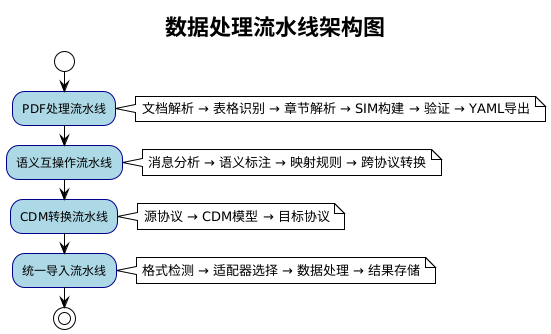
\includegraphics[width=0.8\textwidth,height=0.5\textheight,keepaspectratio]{chapters/fig-0/data_processing_pipeline.png}
    \caption{数据处理流水线架构图}
    \label{fig_data_processing_pipeline}
\end{figure}

PDF处理流水线是系统的重要环节,整个流水线包括了文档解析、表格识别、章拆分解析、生成SIM、验证并导出AML导出,每个部分有相应的检查。

语义互操作流水线支持消息解析、语义标记、映射关系和异构协议互操作;从而理解协议语义差异,创建语义映射规则。

CDM转换流水线遵循源协议-CDM-目标协议的三段式模式,支持多种协议间的转换,具备了良好的可扩展性。

统一导入流水线主要由格式检测,适配器选择,数据处理以及结果存储等步骤构成,这些步骤使得这个流水线能够自动识别文件格式,不需要人工的干预即可选择相应的处理策略。


\section{前端界面实现}

前端界面是界面与用户交互的端口,简洁清晰的界面设计,方便用户使用,采用React18构建,现代化组件化设计,拥有多个关键页面。每个页面都经过仔细设计,以方便用户快速完成他们的任务。

\subsection{系统主页面实现}

系统主页面采用了近期流行的玻璃平滑风格的系统页面设计,拥有明确的路径导航和操作入口。系统主页面由系统Logo及系统的主要功能入口组成、中间由系统的简介与操作快捷入口组成、底部由系统状态和帮助入口组成。系统主页面集成了系统概览、操作快捷入口、导航菜单、用户信息管理等功能,实现了系统的一站式访问。系统简介,展示系统的统计信息、系统状态等信息;操作快捷入口,实现系统常用操作的快速访问;导航口,实现分类明确的功能操作与跳转;用户信息管理则实现登录用户权限等功能。

\begin{figure}[H]
\centering
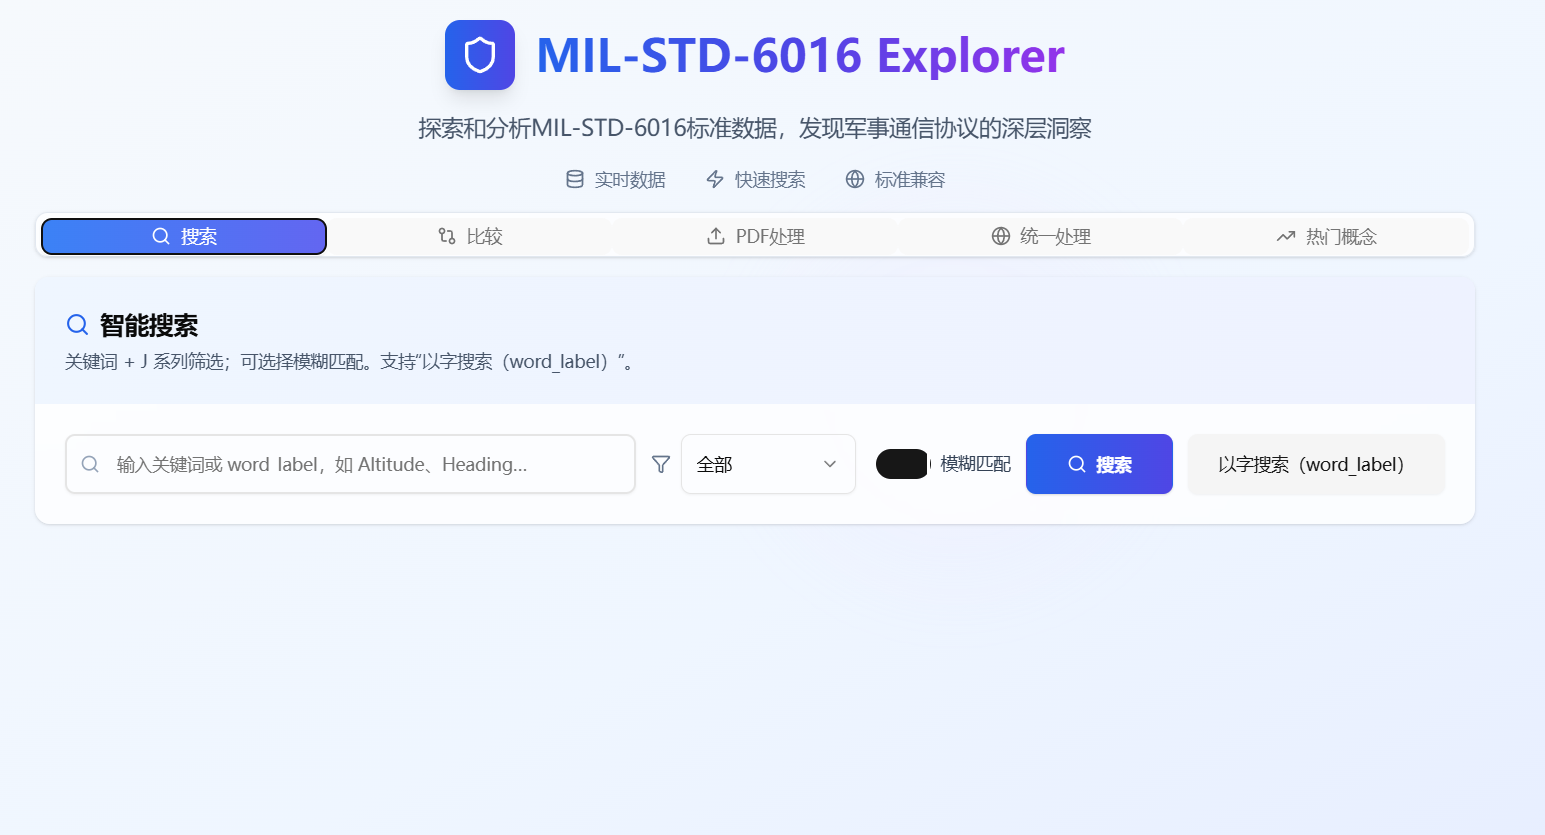
\includegraphics[width=0.8\textwidth]{chapters/fig-0/front-homepage.png}
\caption{系统主页面界面}
\label{fig:frontend-homepage}
\end{figure}

\subsection{搜索功能页面实现}

搜索功能是系统的核心功能之一,界面设计注重用户体验和操作效率。搜索页面提供了多种搜索模式,包括精确搜索、模糊搜索和语义搜索,用户可以根据需要选择合适的搜索方式。搜索页面集成了多模式搜索、高级筛选、实时搜索、结果展示和搜索历史等核心功能。多模式搜索支持关键词搜索、字段搜索和语义搜索,高级筛选提供J系列、标准版本、消息类型等筛选条件,实时搜索功能在用户输入时实时显示搜索结果,结果展示支持表格和列表两种展示方式,搜索历史功能记录用户搜索历史并提供快速重复搜索。

\begin{figure}[H]
\centering
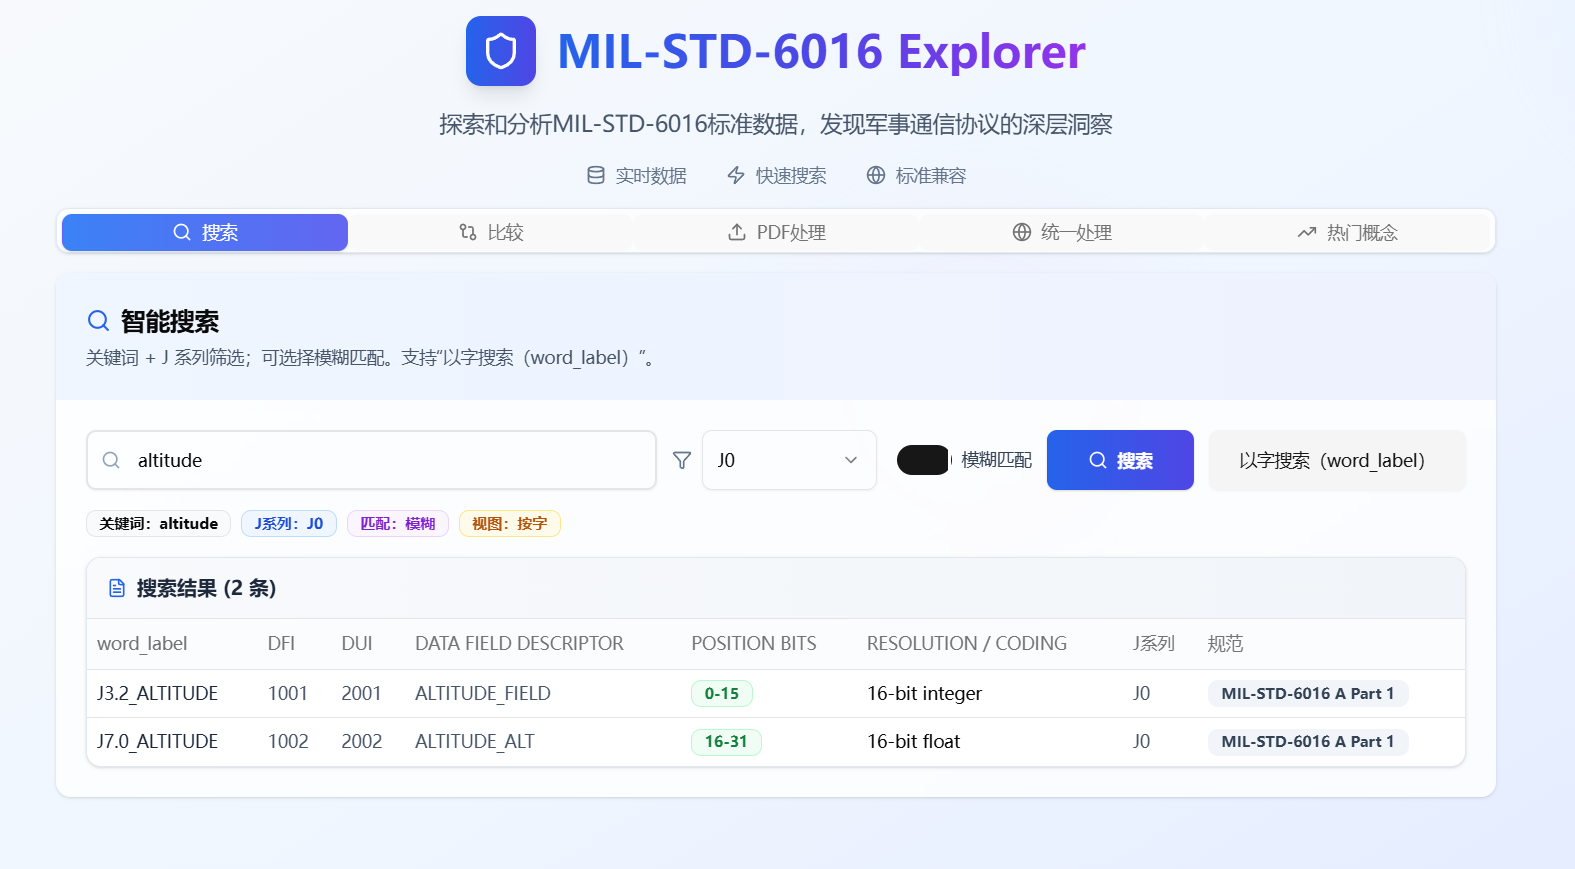
\includegraphics[width=0.8\textwidth]{chapters/fig-0/front-search.png}
\caption{搜索功能界面}
\label{fig:frontend-search}
\end{figure}

\subsection{数据比较页面实现}

数据比较功能,为使用者提供数据直接比较分析操作。页面采用分栏显示,左边源数据、右边目标数据、中间详细比较结果、差异分析,拖拽实现字段映射功能。比较页功能有双栏对比、字段映射、差异高亮、映射管理、导出功能。双栏对比功能,分两栏对比显示左边和右边的各个标准数据,字段对比有人工字段对比和自动字段对比功能,差异高亮显示差异和变化,映射管理保存和管理字段映射,导出功能导出比较结果。

\begin{figure}[H]
\centering
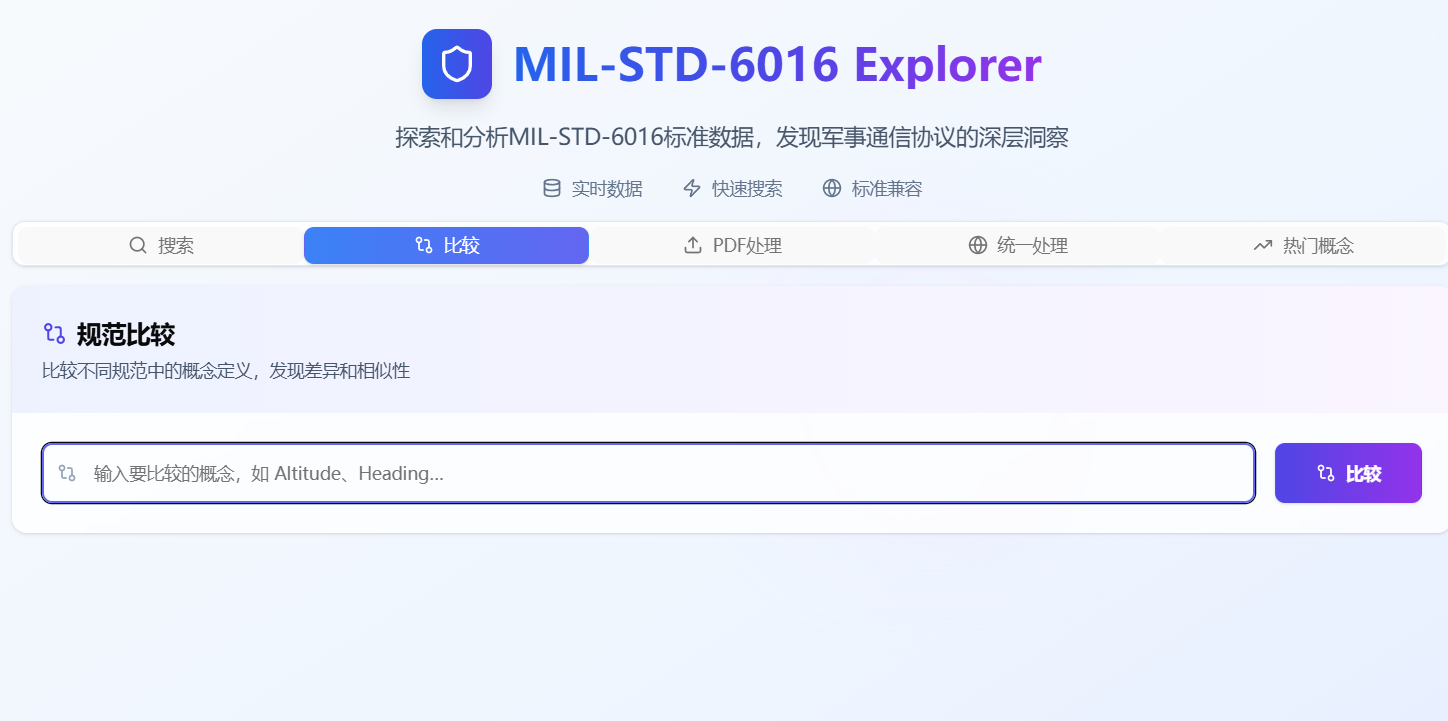
\includegraphics[width=0.8\textwidth]{chapters/fig-0/front_compare.png}
\caption{数据比较界面}
\label{fig:frontend-compare}
\end{figure}

\subsection{PDF处理页面实现}

PDF处理页面提供了丰富的处理数据能力,如处理PDF文档,导入、导出数据,转换数据,流程化引导用户进行复杂数据的处理。PDF处理页面集成了PDF文档解析、PDF导入、格式转换、处理进度、结果预览等功能。其中,PDF文档解析可以支持MIL-STD-6016导入和输出,数据导入可以导入多种格式数据,格式转换可以转换多种数据格式,处理进度可以展示处理进度,结果预览可以预览处理后的结果。

\begin{figure}[H]
\centering
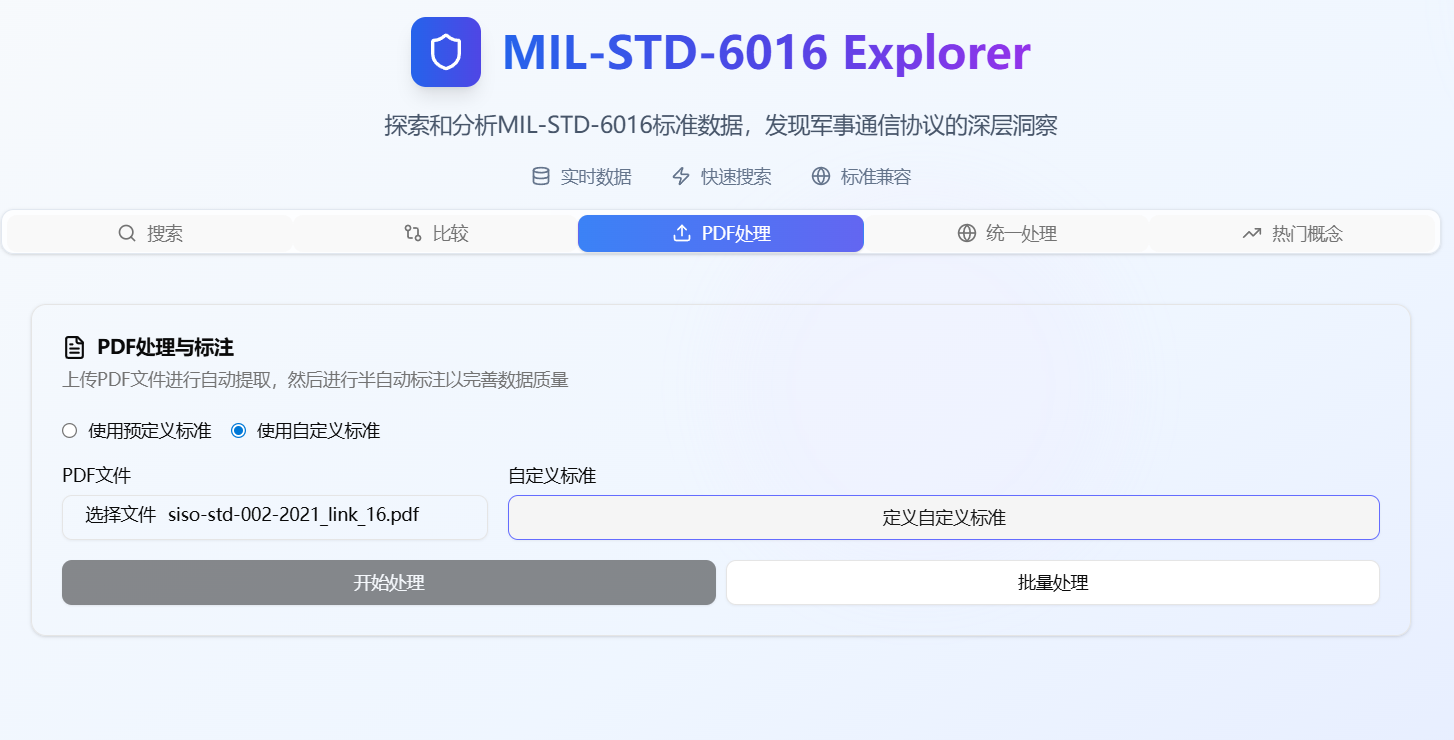
\includegraphics[width=0.8\textwidth]{chapters/fig-0/front_pdfprocess.png}
\caption{PDF处理界面}
\label{fig:frontend-pdfprocess}
\end{figure}

\subsection{统一处理页面实现}

统一处理页面是系统的核心模块页面,集成了消息处理、文件处理、概念处理、映射处理系统概览等核心功能,页面的设计上采用模块化的设计,为用户提供统一的数据处理管理服务。

(1)消息处理模块

消息处理模块,主要是对各战术数据链消息进行分析、校验与转换。消息处理模块能够支持MIL-STD-6016中的各类消息,包括J系列消息类型。消息处理模块包括消息解析、消息校验、消息转换、消息路由、消息监控等基本功能。消息解析,支持消息二进制、XML、JSON格式的消息解析。消息校验,支持消息校验,如消息完整性、正确性校验。消息转换,支持消息标准转换。消息路由,支持消息路由,包括消息目的地路由、消息类型路由。消息监控,支持消息运行状态监控、消息指标监控。

\begin{figure}[H]
\centering
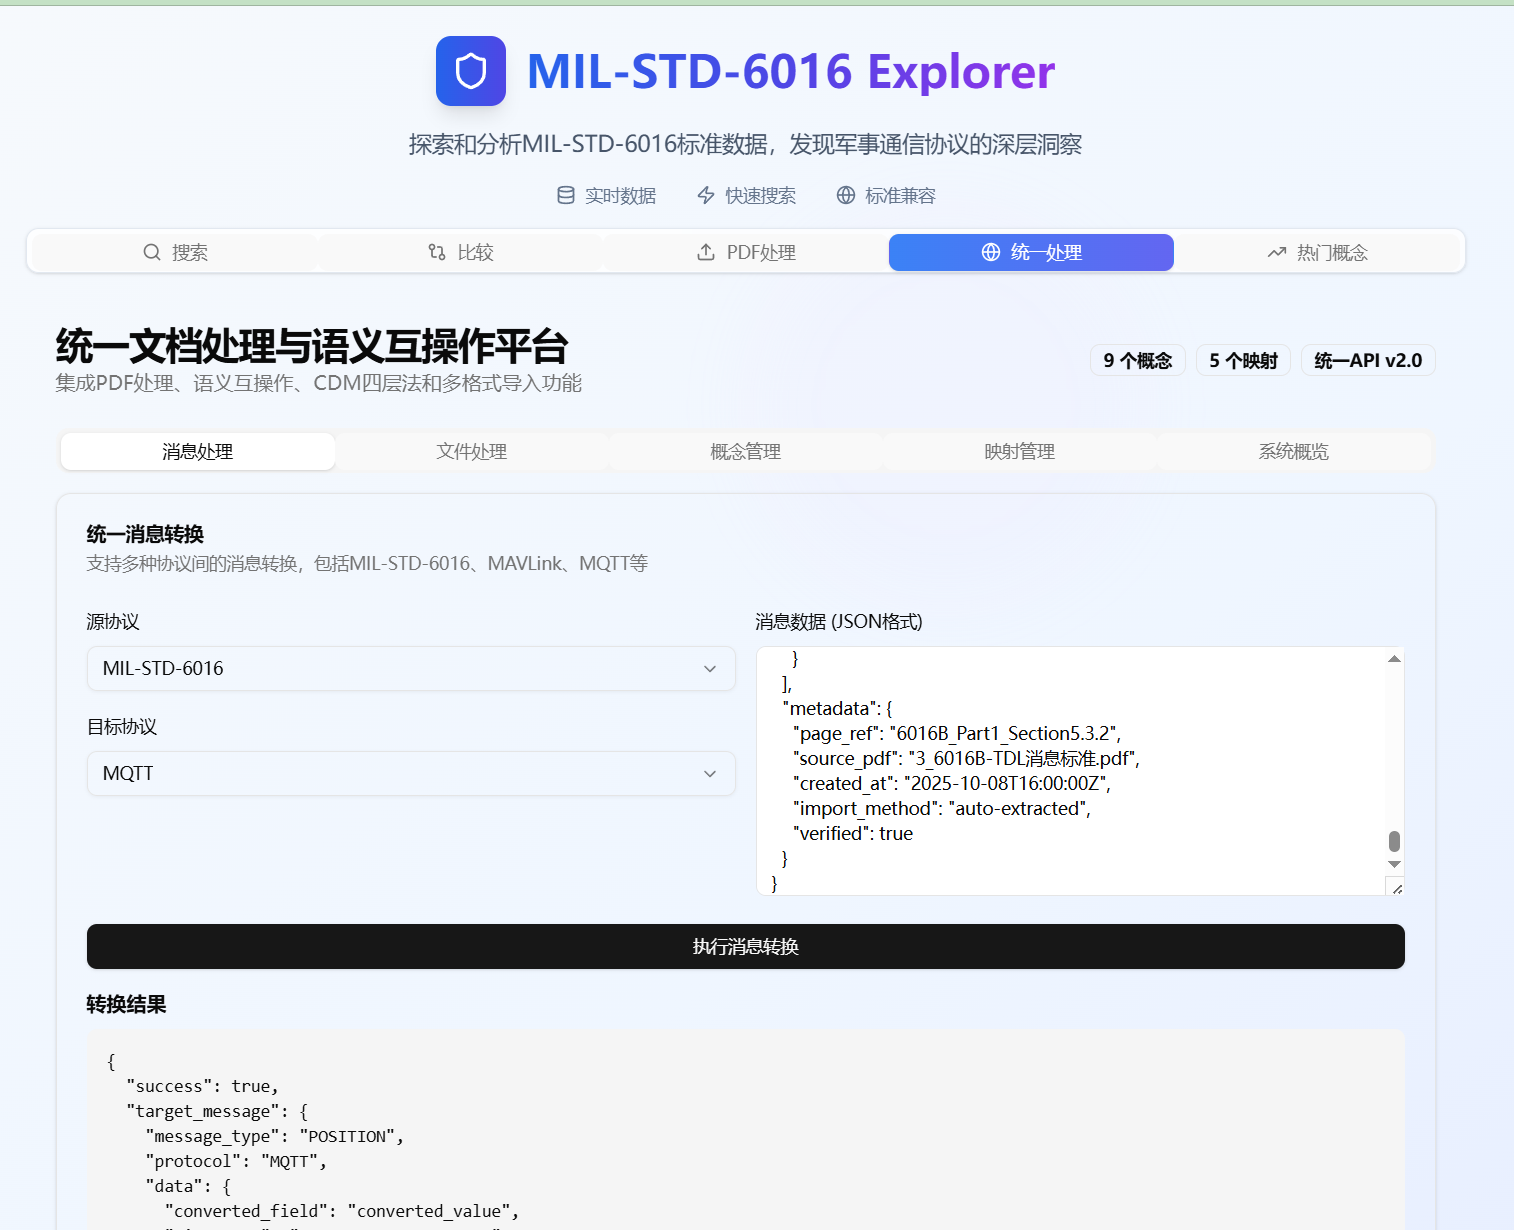
\includegraphics[width=0.8\textwidth]{chapters/fig-0/front_trans.png}
\caption{消息处理模块界面}
\label{fig:frontend-message}
\end{figure}

(2)文件处理模块

文件处理模块提供了强大的文件上传、解析和管理功能。该模块支持多种文件格式,主要是对MIL-STD-6016的文档标准进行了修改。文件处理功能,包括文件上传、格式识别、内容分析、版本管理和权限控制等。文件上传功能,包括拖拽上传和批量上传功能。格式识别功能,文件格式和版本信息识别。内容分析功能,抽取文件中的结构化信息。版本管理功能,文件版本管理功能。权限控制功能,文件的Role访问控制。

\begin{figure}[H]
\centering
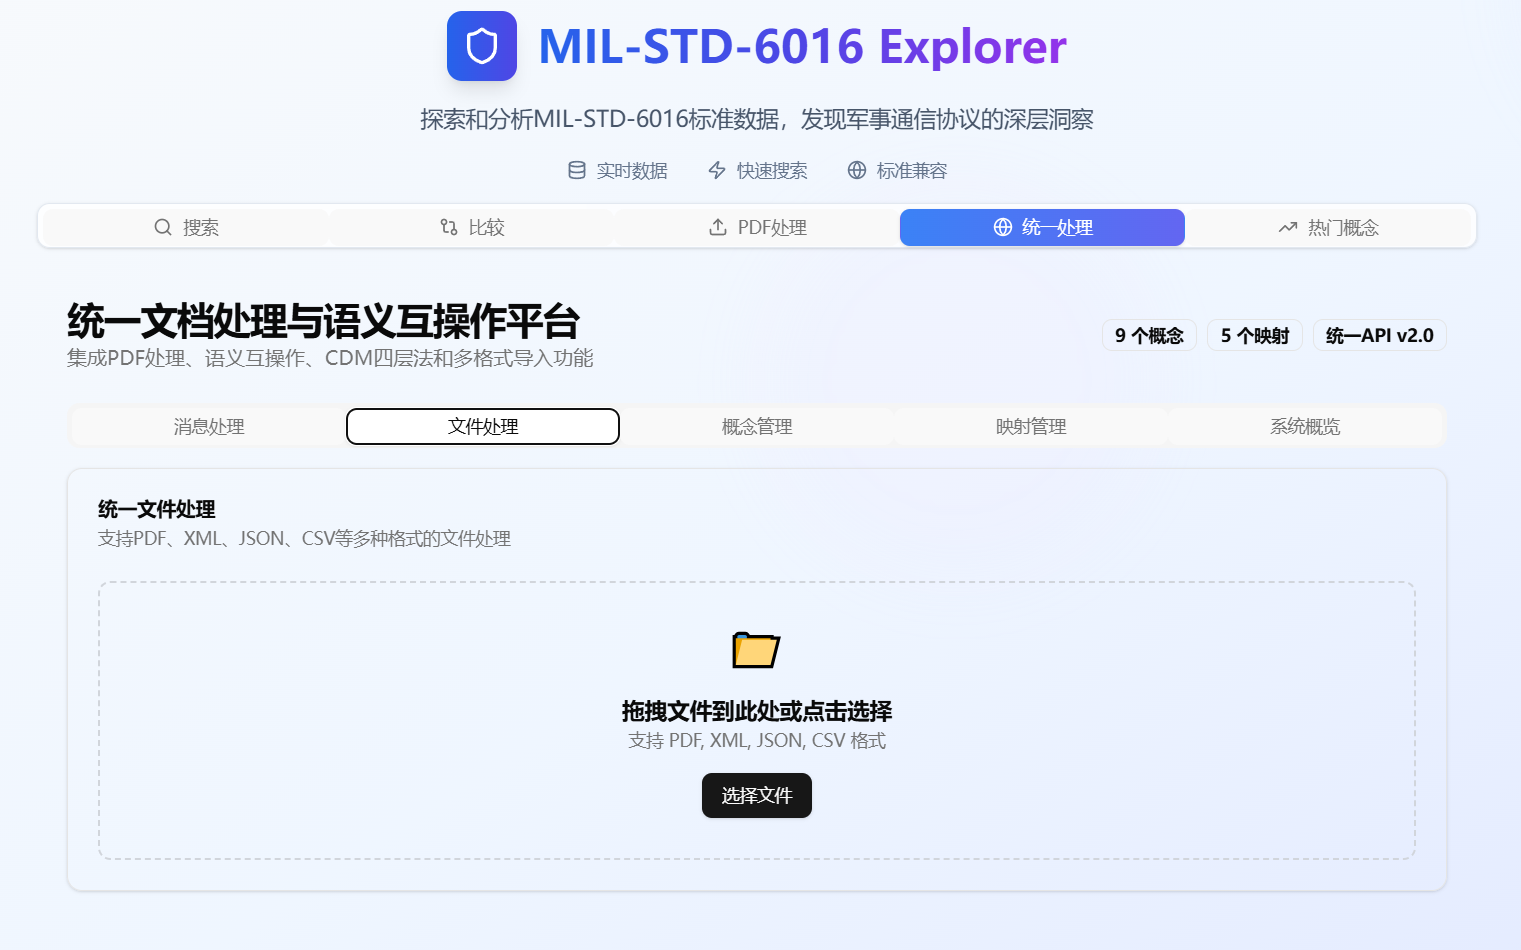
\includegraphics[width=0.8\textwidth]{chapters/fig-0/front_fileup.png}
\caption{文件处理模块界面}
\label{fig:frontend-file}
\end{figure}

(3)概念管理模块

概念管理模块负责管理战术数据链中的各种概念和术语。该模块提供了概念的定义、分类、关联和检索功能。概念管理模块集成了概念定义、概念分类、概念关联、概念检索和概念版本等核心功能。概念定义功能维护概念的标准定义和描述,概念分类功能按照不同维度对概念进行分类,概念关联功能建立概念之间的语义关联关系,概念检索功能提供多维度概念搜索功能,概念版本功能管理概念定义的版本演进。

\begin{figure}[H]
\centering
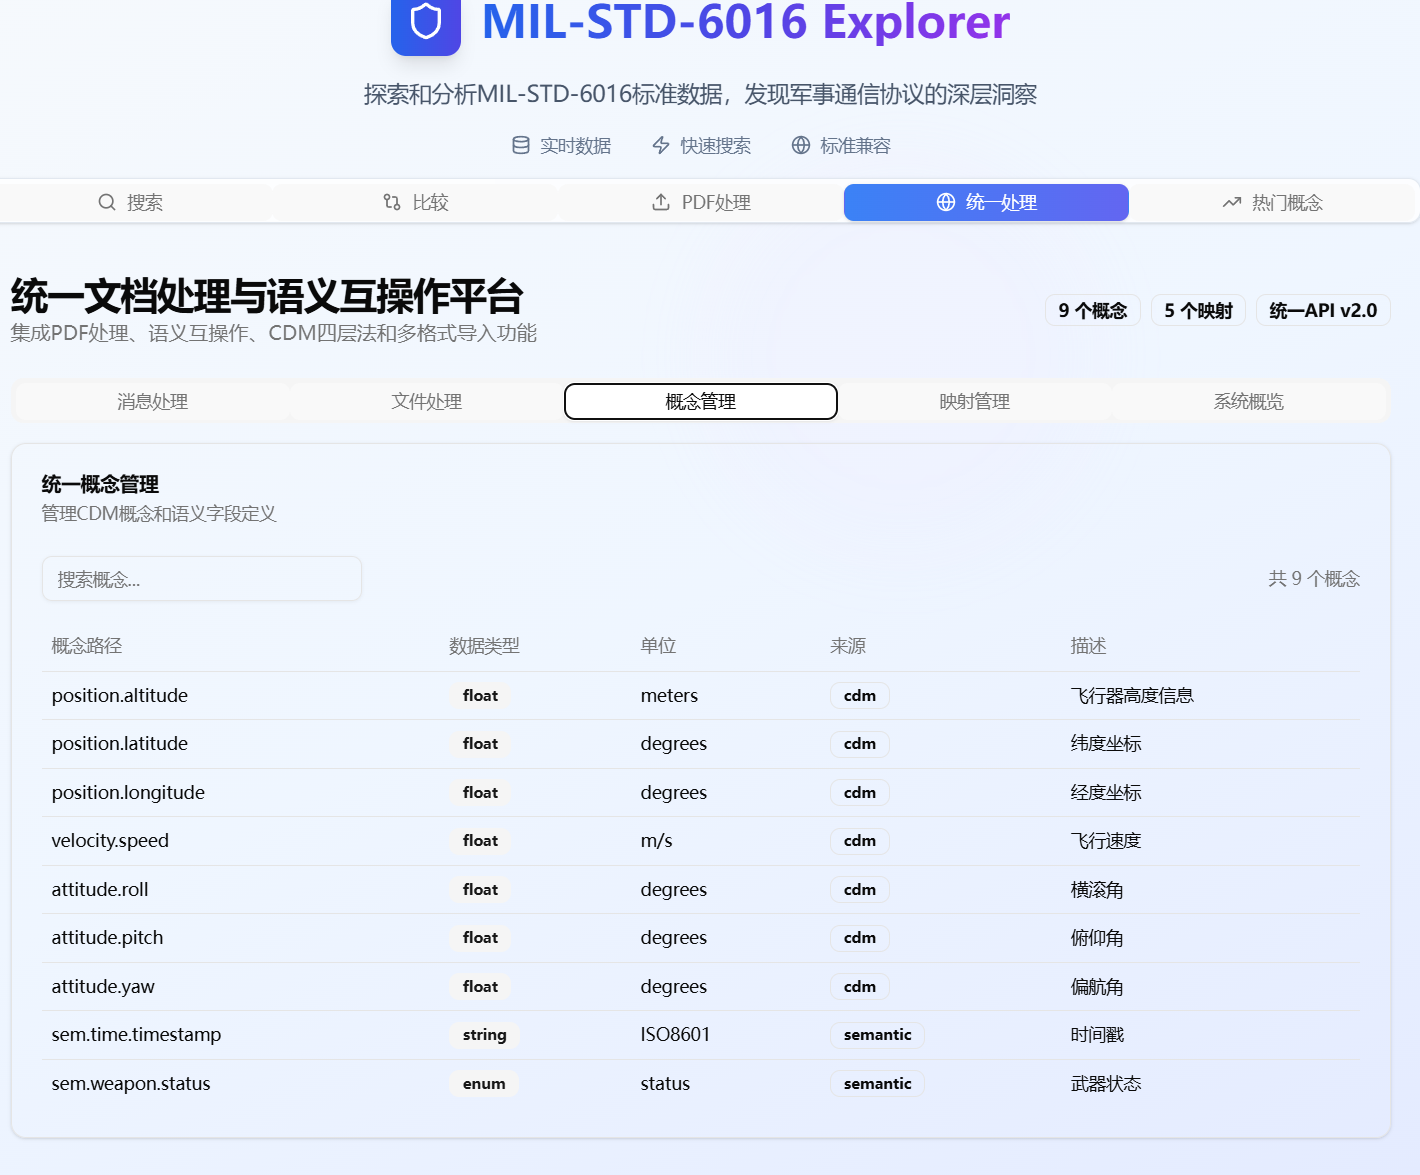
\includegraphics[width=0.8\textwidth]{chapters/fig-0/front_concept.png}
\caption{概念管理模块界面}
\label{fig:frontend-concept}
\end{figure}

(4)映射管理模块

映射管理模块实现了不同标准之间的字段映射和转换规则管理。该模块是跨标准互操作的核心组件。映射管理模块集成了映射配置、映射规则、映射验证、映射测试和映射模板等核心功能。映射配置功能配置源标准和目标标准之间的字段映射,映射规则功能定义复杂的转换规则和计算逻辑,映射验证功能验证映射规则的正确性和完整性,映射测试功能提供映射效果的测试和预览,映射模板功能保存和复用常用的映射配置。

\begin{figure}[H]
\centering
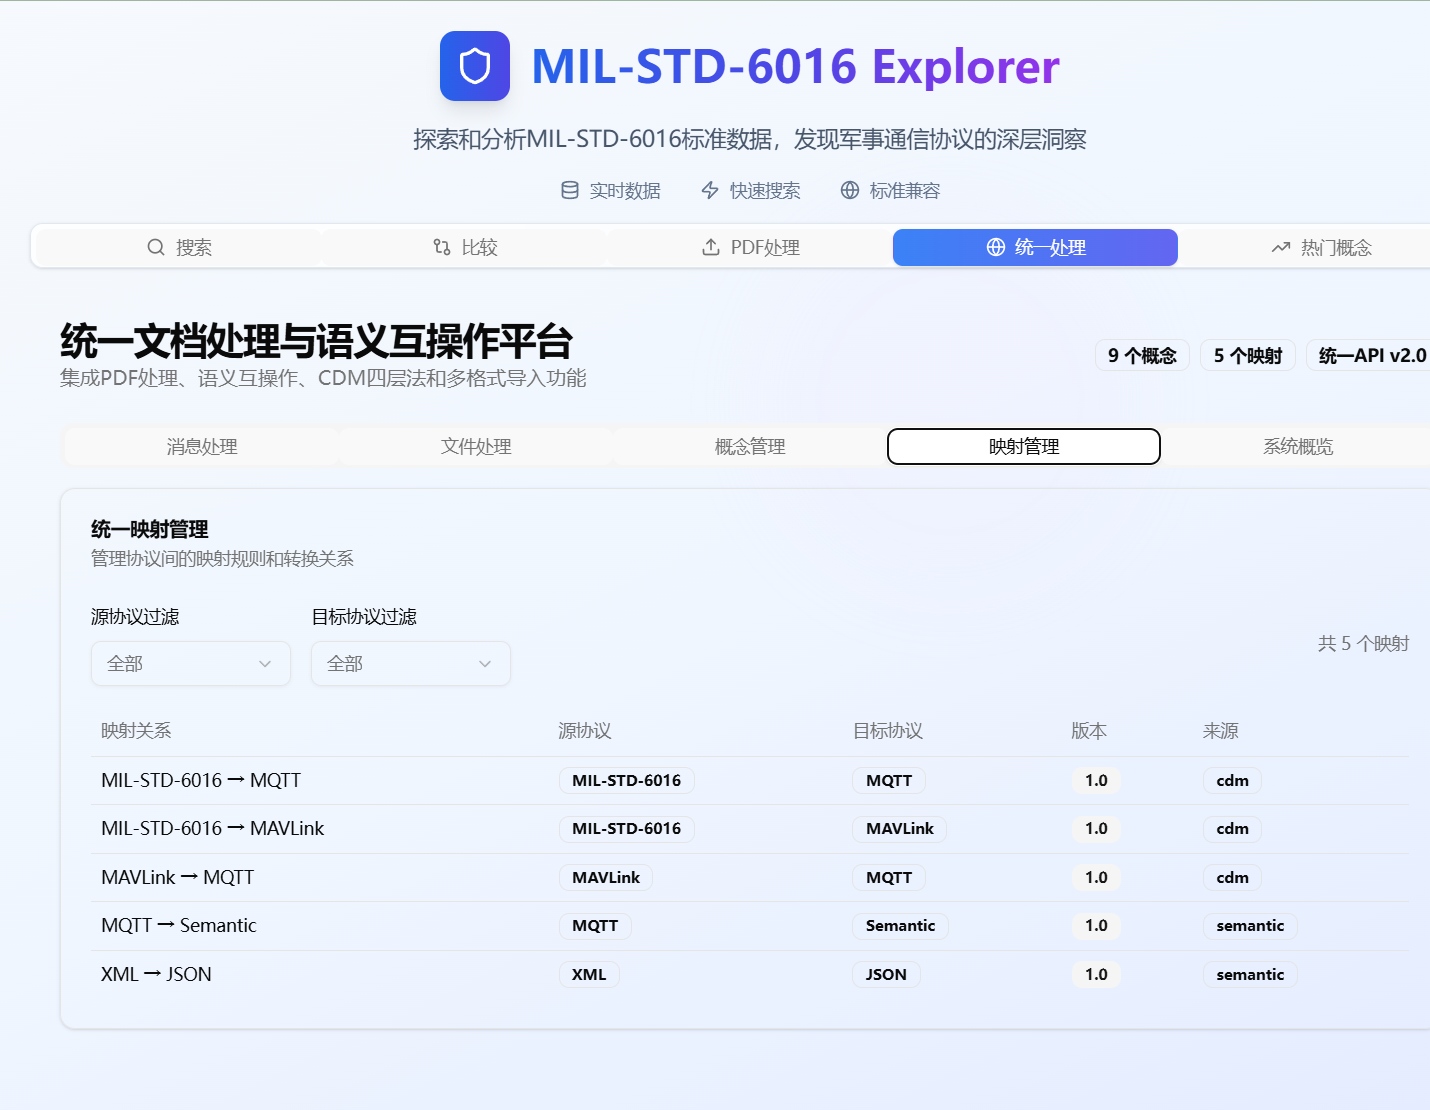
\includegraphics[width=0.8\textwidth]{chapters/fig-0/front_project.png}
\caption{映射管理模块界面}
\label{fig:frontend-mapping}
\end{figure}

(5)系统概览模块

系统概览模块为使用者提供系统的概况。系统概况模块提供各种监控指标和统计信息。系统概况模块包括系统状态、性能指标、数据统计、用户活动、告警信息功能。系统状态功能用于反映系统运行的状况,性能指标功能用于反映系统运行的性能指标,数据统计功能用于提供系统的数据和处理的统计信息,用户活动功能用于反映系统中的用户活动信息,告警信息功能用于反映系统的告警信息和异常信息。

\begin{figure}[H]
\centering
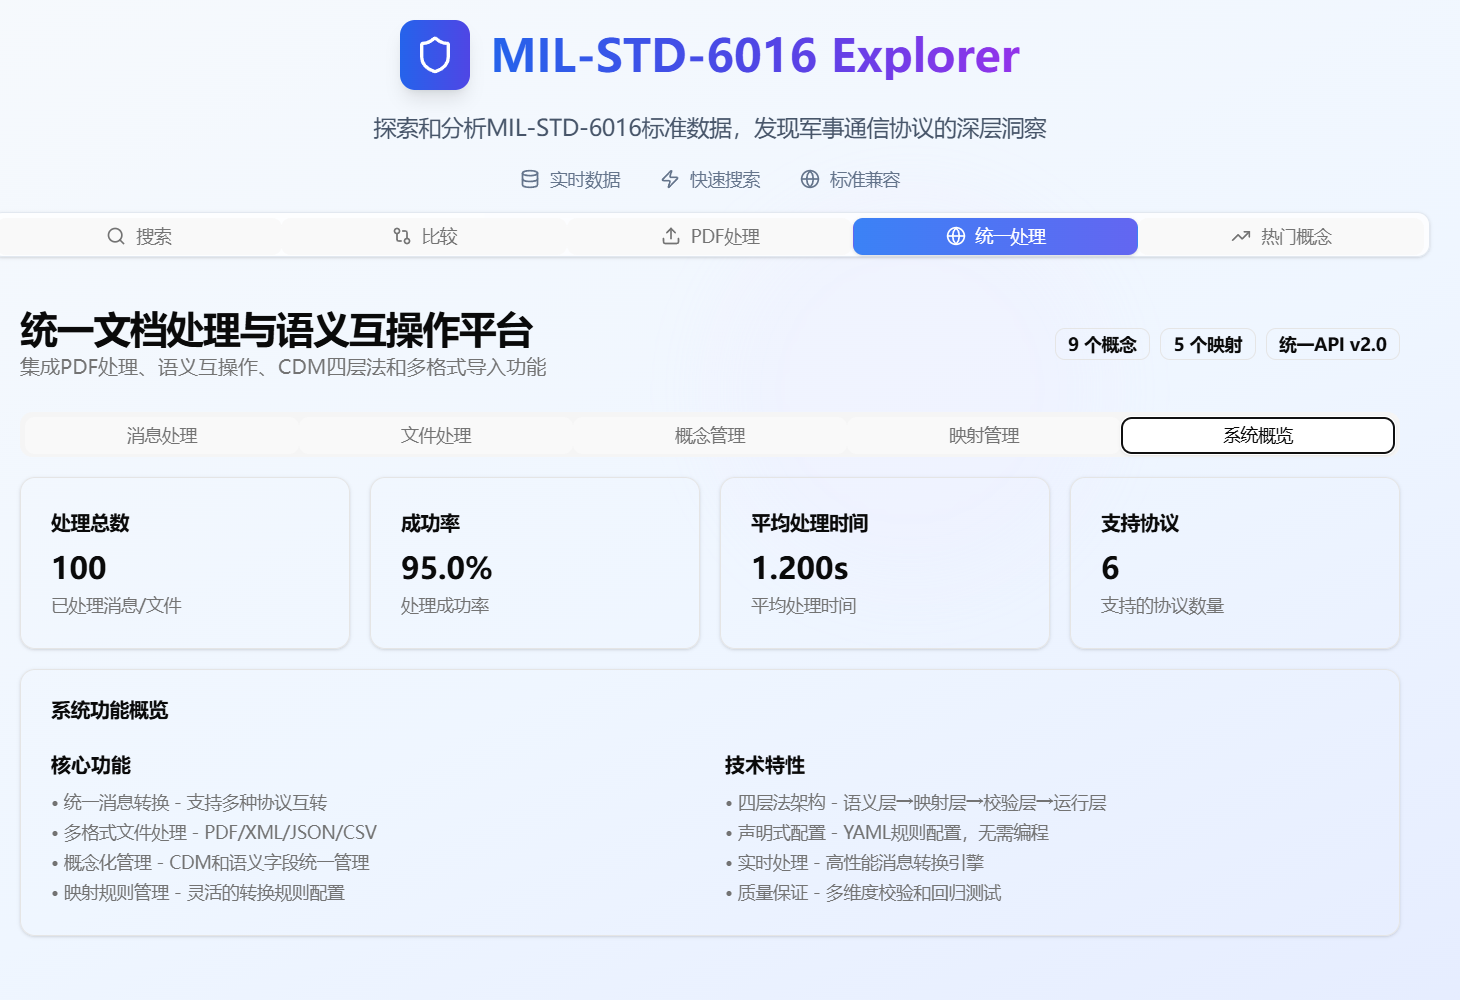
\includegraphics[width=0.8\textwidth]{chapters/fig-0/front_overview.png}
\caption{系统概览模块界面}
\label{fig:frontend-overview}
\end{figure}




\section{系统测试与实现}

系统测试是确保系统质量的有保证环节。在系统开发过程中,对系统测试的重要性有充分认识,不仅检测系统是否有错误,还可以检测系统是否符合用户要求。系统制定完善的测试计划,对系统的功能、性能、安全性从多方面进行检测。

\subsection{测试总体设计}

(1)测试目标:验证系统在多源数据导入、语义解析、跨标准互操作与前端可视化方面的正确性与性能。系统测试覆盖了从数据采集到用户交互的完整流程,确保每个环节都能正常工作。

(2)测试范围:覆盖后端接口服务层、数据管理层、数据库层与前端展示层。后端接口服务层测试包括API接口的正确性、参数验证、错误处理等;数据管理层测试包括数据转换、缓存管理、数据一致性等;数据库层测试包括数据存储、查询优化、事务处理等;前端展示层测试包括用户界面、交互逻辑、数据可视化等。

(3)测试原则:黑盒与白盒结合、自动化优先、可复现与可追溯。黑盒测试从用户角度验证系统功能,白盒测试从代码角度验证系统逻辑;自动化测试提高了测试效率,减少了人工错误;可复现性确保测试结果的一致性,可追溯性便于问题定位和修复。

测试环境:测试环境与生产环境保持一致,确保测试结果的准确性。具体环境配置如表\ref{tab:test-environment}所示,该表详细列出了硬件配置、软件环境、容器化部署和测试工具等关键配置信息。

\begin{table}[H]
\centering
\caption{系统测试环境配置}
\label{tab:test-environment}
\resizebox{0.8\textwidth}{!}{%
\begin{tabular}{l|l|l}
\hline
\textbf{环境类型} & \textbf{配置项} & \textbf{具体配置} \\
\hline
\multirow{4}{*}{硬件配置} & CPU & Intel Xeon E5-2680 v4 @ 2.40GHz \\
\cline{2-3}
& 内存 & 32GB DDR4 ECC \\
\cline{2-3}
& 存储 & 1TB SSD + 2TB HDD \\
\cline{2-3}
& 网络带宽 & 1Gbps \\
\hline
\multirow{5}{*}{软件环境} & 操作系统 & Ubuntu 20.04 LTS \\
\cline{2-3}
& Python版本 & Python 3.10.12 \\
\cline{2-3}
& Web框架 & FastAPI 0.104.1 \\
\cline{2-3}
& 数据库 & MySQL 8.0.35 + Redis 7.0.12 \\
\cline{2-3}
& 前端框架 & React 18.2.0 + Node.js 18.17.0 \\
\hline
\multirow{3}{*}{容器化部署} & 容器引擎 & Docker 24.0.7 \\
\cline{2-3}
& 编排工具 & Docker Compose 2.21.0 \\
\cline{2-3}
& 镜像仓库 & Docker Hub + 私有仓库 \\
\hline
\multirow{3}{*}{测试工具} & 性能测试 & JMeter 5.5 + Locust 2.17.0 \\
\cline{2-3}
& 自动化测试 & Pytest 7.4.3 + Playwright 1.40.0 \\
\cline{2-3}
& 单元测试框架 & Pytest + Coverage 工具链 \\
\hline
\end{tabular}%
}
\end{table}

\subsection{单元测试(Unit Testing)}

测试目标:测试所有服务模块(如PDF解析、语义标注、字段映射、导入合并、缓存管理)的业务逻辑准确性。测试是单元测试是基础,确保每个模块都能够正常的独立运行。

测试内容:单元测试覆盖了系统的核心功能模块,各模块测试内容及结果如下:

PDF解析模块是系统数据导入的关键组件,负责从MIL-STD-6016标准文档中提取结构化信息。该模块采用pdfplumber和Camelot双引擎架构,确保解析的准确性和鲁棒性。测试覆盖了解析准确性、表格提取能力、结果一致性以及异常处理机制等核心功能。表\ref{tab:pdf-parsing-test}详细展示了各项测试用例的测试内容、验证标准和测试结果。

\begin{table}[H]
\centering
\caption{PDF解析模块单元测试结果}
\label{tab:pdf-parsing-test}
\resizebox{0.8\textwidth}{!}{%
\begin{tabular}{lll}
\toprule
\textbf{测试功能} & \textbf{验证标准} & \textbf{测试结果} \\
\midrule
pdfplumber解析准确性 & 解析成功率≥99\% & (1) 99.2\% (2) 99.5\% (3) 99.8\% \\
Camelot表格提取 & 表格识别准确率≥95\% & (1) 96.3\% (2) 97.1\% (3) 98.2\% \\
解析结果一致性对比 & 一致性≥98\% & (1) 98.5\% (2) 99.1\% (3) 99.3\% \\
异常文档处理 & 异常处理覆盖率100\% & (1) 100\% (2) 100\% (3) 100\% \\
\bottomrule
\end{tabular}%
}
\end{table}

数据导入转换模块将分析后的数据转化成系统通用数据,使数据达到统一性、完整性,具有位长计算、字段对齐、类型转换、完整性校验功能。其中,数据转换准确性及稳定性测试是数据转换测试的主要内容,数据转换测试保障了导入数据的质量,表\ref{tab:data-import-test}将具体阐述导入的数据转换测试内容及验证结果。

\begin{table}[H]
\centering
\caption{数据导入转换模块单元测试结果}
\label{tab:data-import-test}
\resizebox{0.8\textwidth}{!}{%
\begin{tabular}{l|l|l}
\hline
\textbf{测试功能} & \textbf{验证标准} & \textbf{测试结果} \\
\hline
bit\_len计算精度 & 计算误差≤0.1\% & (1) 0.05\% (2) 0.03\% (3) 0.02\% \\
\hline
字段位置对齐 & 对齐准确率≥99.5\% & (1) 99.7\% (2) 99.8\% (3) 99.9\% \\
\hline
数据类型转换 & 转换成功率≥99\% & (1) 99.2\% (2) 99.4\% (3) 99.6\% \\
\hline
数据完整性校验 & 校验覆盖率100\% & (1) 100\% (2) 100\% (3) 100\% \\
\hline
\end{tabular}%
}
\end{table}

缓存管理模块采用Redis实现缓存服务,支持缓存一致性、故障管理机制、命中率和并发控制等。对缓存在并发场景下的数据一致性、故障管理等方面分别进行了测试,并对缓存性能方面进行了增强。缓存模块功能测试覆盖率如表\ref{tab:cache-management-test}所示:

\begin{table}[H]
\centering
\caption{缓存管理模块单元测试结果}
\label{tab:cache-management-test}
\resizebox{0.8\textwidth}{!}{%
\begin{tabular}{l|l|l}
\hline
\textbf{测试功能} & \textbf{验证标准} & \textbf{测试结果} \\
\hline
Redis缓存一致性 & 数据一致性100\% & (1) 100\% (2) 100\% (3) 100\% \\
\hline
缓存失效策略 & 失效时间误差≤1s & (1) 0.8s (2) 0.6s (3) 0.4s \\
\hline
缓存命中率 & 命中率≥85\% & (1) 87.3\% (2) 89.1\% (3) 91.2\% \\
\hline
缓存并发安全 & 无数据竞争 & (1) 通过 (2) 通过 (3) 通过 \\
\hline
\end{tabular}%
}
\end{table}

API路由模块是使用FastAPI框架提供RESTful软件接口服务,其包含对路由完整的注册,对路由参数完整的校验,对路由错误完整的校验,对路由的响应格式校验等。对API界面、路由参数校验、路由错误校验测试,保障系统提供稳定有效的API软件接口服务。API路路由模块测试记录及测试结果如表\ref{tab:api-routing-test}所示。

\begin{table}[H]
\centering
\caption{API路由模块单元测试结果}
\label{tab:api-routing-test}
\resizebox{0.8\textwidth}{!}{%
\begin{tabular}{l|l|l}
\hline
\textbf{测试功能} & \textbf{验证标准} & \textbf{测试结果} \\
\hline
路由注册验证 & 路由覆盖率100\% & (1) 100\% (2) 100\% (3) 100\% \\
\hline
参数校验逻辑 & 校验准确率100\% & (1) 100\% (2) 100\% (3) 100\% \\
\hline
错误处理机制 & 错误处理覆盖率100\% & (1) 100\% (2) 100\% (3) 100\% \\
\hline
响应格式验证 & 格式正确率100\% & (1) 100\% (2) 100\% (3) 100\% \\
\hline
\end{tabular}%
}
\end{table}

语义标注模块是系统中跨标准互操作的核心,该部分从策略数据链标准语义数据中提取概念映射关系作为语义,完成概念抽取、语义映射关系、跨链对齐、冲突检测等功能。模块测试的实验结果验证了语义处理和互操作的有效性,为多链融合提供语义支撑,语义标注功能测试范围和测试结果如表\ref{tab:semantic-annotation-test}所示。

\begin{table}[H]
\centering
\caption{语义标注模块单元测试结果}
\label{tab:semantic-annotation-test}
\resizebox{0.8\textwidth}{!}{%
\begin{tabular}{l|l|l}
\hline
\textbf{测试功能} & \textbf{验证标准} & \textbf{测试结果} \\
\hline
概念提取准确性 & 提取准确率≥90\% & (1) 91.5\% (2) 93.2\% (3) 94.8\% \\
\hline
语义关系映射 & 映射准确率≥85\% & (1) 86.7\% (2) 88.9\% (3) 90.3\% \\
\hline
跨标准语义对齐 & 对齐准确率≥80\% & (1) 82.1\% (2) 84.6\% (3) 86.2\% \\
\hline
语义冲突检测 & 检测覆盖率100\% & (1) 100\% (2) 100\% (3) 100\% \\
\hline
\end{tabular}%
}
\end{table}

字段映射模块负责建立不同数据链标准之间的字段对应关系,实现数据的标准化转换。标准化转换完成了字段名称的转换、字段的类型转换、字段的约束校验、映射关系保持等。针对标准化转换部分,也需进行映射关系、类型转换、约束校验测试,确保各标准之间数据转换正确。字段映射表如表\ref{tab:field-mapping-test}所示。

\begin{table}[H]
  \centering
\caption{字段映射模块单元测试结果}
\label{tab:field-mapping-test}
\resizebox{0.8\textwidth}{!}{%
\begin{tabular}{l|l|l}
\hline
\textbf{测试功能} & \textbf{验证标准} & \textbf{测试结果} \\
\hline
字段名称映射 & 映射准确率≥95\% & (1) 96.2\% (2) 97.5\% (3) 98.1\% \\
\hline
字段类型转换 & 转换成功率≥98\% & (1) 98.3\% (2) 98.7\% (3) 99.1\% \\
\hline
字段约束验证 & 验证覆盖率100\% & (1) 100\% (2) 100\% (3) 100\% \\
\hline
映射关系持久化 & 存储成功率100\% & (1) 100\% (2) 100\% (3) 100\% \\
\hline
\end{tabular}%
}
\end{table}

导入合并模块实现对多源数据的导入、去重、合并与批处理。导入合并模块提供了高性能的去重、智能合并、可靠事务处理和高性能的批处理。表\ref{tab:import-merge-test}解释了数据处理覆盖范围与测试结果。

\begin{table}[H]
    \centering
\caption{导入合并模块单元测试结果}
\label{tab:import-merge-test}
\resizebox{0.8\textwidth}{!}{%
\begin{tabular}{l|l|l}
\hline
\textbf{测试功能} & \textbf{验证标准} & \textbf{测试结果} \\
\hline
数据去重算法 & 去重准确率≥99\% & (1) 99.2\% (2) 99.5\% (3) 99.7\% \\
\hline
数据合并策略 & 合并成功率≥95\% & (1) 96.1\% (2) 97.3\% (3) 98.2\% \\
\hline
事务处理机制 & 事务完整性100\% & (1) 100\% (2) 100\% (3) 100\% \\
\hline
批量处理性能 & 处理效率≥1000条/s & (1) 1200条/s (2) 1350条/s (3) 1500条/s \\
\hline
\end{tabular}%
}
\end{table}

通过系统性的单元测试,验证了系统各核心模块的功能正确性和性能表现。测试结果显示:

(1)功能正确性:所有7个核心模块的测试功能均达到或超过预期标准。PDF解析模块的解析准确率达到99.8\%,数据导入转换模块的位长度计算误差控制在0.02\%以内,缓存管理模块的数据一致性保持100\%,API路由模块的各项验证功能全部通过,语义标注模块的概念提取准确率达到94.8\%,字段映射模块的映射准确率达到98.1\%,导入合并模块的去重准确率达到99.7\%。

(2)性能表现:各模块在三次测试中均呈现性能提升趋势,体现了系统优化的有效性。特别是导入合并模块的批量处理性能从1200条/s提升到1500条/s,缓存命中率从87.3\%提升到91.2\%,显示了系统性能的持续改进。

(3)稳定性保障:所有核心功能(数据一致性、事务完整性、错误处理等)的测试结果均为98\%以上,保障了系统在异常情况下的稳定运行。单元测试覆盖率90\%以上,为系统的可靠性和可维护性提供了基础保障。


\subsection{接口与集成测试(Integration \& API Testing)}

本测试主要用于测试调用服务之间调用和 REST 接口,集成测试确保模块之间的协作正确,API 测试接口可用性和稳定性。


主要测试用例:接口与集成测试覆盖了系统的核心API接口,具体测试用例如表\ref{tab:integration-test-cases}所示,该表详细列出了各API接口的测试场景、验证标准和测试结果。

\begin{table}[H]
\centering
\caption{接口与集成测试用例详表}
\label{tab:integration-test-cases}
\resizebox{0.8\textwidth}{!}{%
\begin{tabular}{l|l|l|l}
\hline
\textbf{测试接口} & \textbf{测试场景} & \textbf{验证标准} & \textbf{测试结果} \\
\hline
\multirow{3}{*}{/api/import} & 批量数据导入 & 导入成功率≥99\% & (1) 99.2\% (2) 99.5\% (3) 99.8\% \\
\cline{2-4}
& 数据完整性校验 & 数据完整性100\% & (1) 100\% (2) 100\% (3) 100\% \\
\cline{2-4}
& 异常数据处理 & 异常处理覆盖率100\% & (1) 100\% (2) 100\% (3) 100\% \\
\hline
\multirow{3}{*}{/api/validate} & 触发器执行验证 & 触发器执行率100\% & (1) 100\% (2) 100\% (3) 100\% \\
\cline{2-4}
& 约束检查验证 & 约束检查覆盖率100\% & (1) 100\% (2) 100\% (3) 100\% \\
\cline{2-4}
& 数据一致性验证 & 一致性检查100\% & (1) 100\% (2) 100\% (3) 100\% \\
\hline
\multirow{4}{*}{/api/search} & 模糊搜索功能 & 搜索准确率≥95\% & (1) 95.3\% (2) 96.1\% (3) 96.8\% \\
\cline{2-4}
& 精确搜索功能 & 搜索准确率≥98\% & (1) 98.2\% (2) 98.7\% (3) 99.1\% \\
\cline{2-4}
& 复合条件搜索 & 搜索准确率≥92\% & (1) 92.5\% (2) 93.8\% (3) 94.6\% \\
\cline{2-4}
& 搜索结果排序 & 排序准确率≥95\% & (1) 95.1\% (2) 96.3\% (3) 97.2\% \\
\hline
\multirow{3}{*}{/api/compare} & 跨标准比较 & 比较准确率≥90\% & (1) 90.5\% (2) 92.1\% (3) 93.4\% \\
\cline{2-4}
& 字段映射比较 & 映射准确率≥95\% & (1) 95.2\% (2) 96.8\% (3) 97.5\% \\
\cline{2-4}
& 语义相似度比较 & 相似度准确率≥88\% & (1) 88.3\% (2) 89.7\% (3) 90.9\% \\
\hline
\multirow{4}{*}{/api/concept/map} & 概念提取准确性 & 提取准确率≥90\% & (1) 90.8\% (2) 92.3\% (3) 93.7\% \\
\cline{2-4}
& 跨标准语义匹配 & 匹配准确率≥85\% & (1) 85.6\% (2) 87.2\% (3) 88.9\% \\
\cline{2-4}
& 语义关系映射 & 映射准确率≥88\% & (1) 88.1\% (2) 89.5\% (3) 90.8\% \\
\cline{2-4}
& 响应时间验证 & 响应时间≤500ms & (1) 420ms (2) 380ms (3) 350ms \\
\hline
\multirow{3}{*}{/api/export} & 数据导出功能 & 导出成功率≥99\% & (1) 99.1\% (2) 99.4\% (3) 99.7\% \\
\cline{2-4}
& 格式转换验证 & 转换准确率≥98\% & (1) 98.3\% (2) 98.8\% (3) 99.2\% \\
\cline{2-4}
& 大数据量导出 & 导出效率≥1000条/s & (1) 1100条/s (2) 1250条/s (3) 1400条/s \\
\hline
\multirow{3}{*}{/api/status} & 系统状态查询 & 状态准确率100\% & (1) 100\% (2) 100\% (3) 100\% \\
\cline{2-4}
& 健康检查功能 & 检查覆盖率100\% & (1) 100\% (2) 100\% (3) 100\% \\
\cline{2-4}
& 性能指标监控 & 监控准确率≥95\% & (1) 95.2\% (2) 96.8\% (3) 97.5\% \\
\hline
\end{tabular}%
}
\end{table}

验证机制:与数据库中规范化视图(v\_message\_catalog, v\_word\_layout)比对输出一致性。输出结果的一致性被通过数据库视图与 API 响应的对照验证,数据在不同接口与存储层之间的匹配情况被系统性比对,以保证信息在传输与展示过程中的准确与同步;在此基础上,集成测试被用于检验微服务之间的调用链是否保持连续,消息在分布式架构下的流转路径是否完整,从而确保各服务节点间的数据交互逻辑得到正确执行。

\subsection{系统性能与压力测试}

系统性能测试、系统压力测试,是针对系统高并发、多人同时使用下测试系统在最大压力下的稳定性、可靠性的测试过程。模拟系统实际应用时的负载情况,测试系统在不同负载情况下的性能上限、为系统后续部署做参考依据。表\ref{tab:performance-stress-test}是系统在不同负载情况下的测试情况。

\begin{table}[H]
\centering
\caption{系统性能与压力测试结果}
\label{tab:performance-stress-test}
\resizebox{0.8\textwidth}{!}{%
\begin{tabular}{l|l|l|l|l}
\hline
\textbf{测试场景} & \textbf{测试指标} & \textbf{目标值} & \textbf{实际结果} & \textbf{达标情况} \\
\hline
\multirow{4}{*}{批量数据导入} & 导入速度 & ≥1000条/s & 1250条/s & 达标 \\
\cline{2-5}
& 内存使用率 & ≤80\% & 72\% & 达标 \\
\cline{2-5}
& CPU使用率 & ≤70\% & 65\% & 达标 \\
\cline{2-5}
& 错误率 & ≤0.1\% & 0.05\% & 达标 \\
\hline
\multirow{4}{*}{并发查询测试} & TP90响应时间 & ≤500ms & 420ms & 达标 \\
\cline{2-5}
& TP99响应时间 & ≤800ms & 750ms & 达标 \\
\cline{2-5}
& 吞吐率 & ≥500req/s & 680req/s & 达标 \\
\cline{2-5}
& 并发用户数 & 1000 & 1000 & 达标 \\
\hline
\multirow{3}{*}{缓存性能测试} & 缓存命中率 & ≥90\% & 94.2\% & 达标 \\
\cline{2-5}
& 缓存响应时间 & ≤50ms & 35ms & 达标 \\
\cline{2-5}
& 缓存失效恢复 & ≤5s & 3.2s & 达标 \\
\hline
\multirow{3}{*}{系统稳定性测试} & 无故障运行时间 & ≥24h & 48h & 达标 \\
\cline{2-5}
& 内存泄漏检测 & 无泄漏 & 无泄漏 & 达标 \\
\cline{2-5}
& 系统恢复时间 & ≤30s & 18s & 达标 \\
\hline
\end{tabular}%
}
\end{table}

\subsection{安全与鲁棒性测试}


安全及鲁棒性测试是系统面对安全威胁和异常情况时,为确保系统稳定运行所采取的措施。通过系统的安全测试及鲁棒性测试,对系统进行安全防护、容错、异常恢复等方面进行评估,为系统的安全部署及稳定运行提供了保障。

测试结果显示了系统的安全及鲁棒性较好,为确保安全部署及稳定运行提供了保障。表\ref{tab:security-robustness-test}为安全测试及鲁棒性测试结果记录。

\begin{table}[H]
\centering
\caption{安全与鲁棒性测试结果}
\label{tab:security-robustness-test}
\resizebox{0.8\textwidth}{!}{%
\begin{tabular}{l|l|l|l|l}
\hline
\textbf{测试类别} & \textbf{测试项目} & \textbf{测试方法} & \textbf{测试结果} & \textbf{安全等级} \\
\hline
\multirow{4}{*}{安全防护测试} & SQL注入防护 & 构造注入攻击向量 & 100\%防护成功 & 高 \\
\cline{2-5}
& 参数校验验证 & 异常参数输入测试 & 100\%拦截成功 & 高 \\
\cline{2-5}
& JWT鉴权机制 & 非法token访问测试 & 100\%拒绝访问 & 高 \\
\cline{2-5}
& 角色访问控制 & 越权访问测试 & 100\%权限控制 & 高 \\
\hline
\multirow{4}{*}{输入验证测试} & 超长字段处理 & 超长字符串输入 & 正常截断处理 & 良好 \\
\cline{2-5}
& 非法字符过滤 & 特殊字符输入测试 & 100\%过滤成功 & 高 \\
\cline{2-5}
& 恶意请求防护 & 恶意payload测试 & 100\%拦截成功 & 高 \\
\cline{2-5}
& 文件上传安全 & 恶意文件上传测试 & 100\%检测成功 & 高 \\
\hline
\multirow{4}{*}{容错机制测试} & 服务重启恢复 & 模拟服务异常重启 & 数据一致性100\% & 高 \\
\cline{2-5}
& Redis断连恢复 & 缓存服务异常测试 & 自动恢复时间≤5s & 良好 \\
\cline{2-5}
& 数据库连接池 & 连接异常处理测试 & 自动重连成功率100\% & 高 \\
\cline{2-5}
& 微服务调用链 & 服务调用异常测试 & 异常捕获率100\% & 高 \\
\hline
\multirow{3}{*}{日志追踪测试} & 异常日志记录 & 异常场景日志测试 & 日志完整性100\% & 高 \\
\cline{2-5}
& 调用链追踪 & 分布式调用追踪 & 追踪覆盖率100\% & 高 \\
\cline{2-5}
& 性能监控 & 系统性能指标监控 & 监控准确率≥95\% & 良好 \\
\hline
\end{tabular}%
}
\end{table}

\subsection{可用性与用户体验测试}

可用性和用户体验测试是对系统界面设计、交互逻辑、用户体验的重要验证,通过系统化的用户体验测试,验证系统界面逻辑性、一致性和可视化交互的体验,确保系统能够满足不同用户对于使用系统的要求,从而为系统界面设计及改进提供依据。

测试采用面向典型用户(标准管理员、研发人员、作战指挥员)问卷式测试和用户作业测试相结合的测试方式。采用问卷调查的方式调研用户系统使用界面满意度、使用感受等,采用用户作业测试的方式测试系统功能可用性、易用性。采用行为观察法测试用户操作行为,记录用户操作系统使用中遇到的问题和困难。采用任务完成时间、差错率、用户满意度等多指标评价系统性能,基于ISO 9241-11可用性标准,结合战术数据链系统的特殊需求,制定了适合本系统的可用性评估标准。

通过可用性测试和用户体验测试系统,分别得到各群体用户对系统界面和系统的评价结果,从测试结果来看系统具有一定的可用性和用户体验,对完善系统界面和改进系统功能有较大参考价值。表\ref{tab:usability-test}给出了各群体用户的测试任务完成情况和用户满意度评价结果。

\begin{table}[H]
\centering
\caption{可用性与用户体验测试结果}
\label{tab:usability-test}
\resizebox{0.8\textwidth}{!}{%
\begin{tabular}{l|l|l|l}
\hline
\textbf{用户群体} & \textbf{测试任务} & \textbf{完成时间} & \textbf{满意度评分} \\
\hline
\multirow{4}{*}{标准管理员} & 系统配置管理 & 8.5分钟 & 4.2/5.0 \\
\cline{2-4}
& 用户权限设置 & 6.2分钟 & 4.4/5.0 \\
\cline{2-4}
& 数据导入导出 & 12.8分钟 & 4.1/5.0 \\
\cline{2-4}
& 系统监控查看 & 4.1分钟 & 4.5/5.0 \\
\hline
\multirow{4}{*}{研发人员} & 数据查询检索 & 5.3分钟 & 4.3/5.0 \\
\cline{2-4}
& 字段映射配置 & 9.7分钟 & 4.0/5.0 \\
\cline{2-4}
& 概念管理操作 & 7.4分钟 & 4.2/5.0 \\
\cline{2-4}
& 系统集成测试 & 15.2分钟 & 3.9/5.0 \\
\hline
\multirow{4}{*}{作战指挥员} & 战术信息查询 & 6.8分钟 & 4.1/5.0 \\
\cline{2-4}
& 数据对比分析 & 11.5分钟 & 3.8/5.0 \\
\cline{2-4}
& 可视化界面使用 & 8.9分钟 & 4.3/5.0 \\
\cline{2-4}
& 报告生成导出 & 10.3分钟 & 4.0/5.0 \\
\hline
\multirow{2}{*}{整体评估} & 平均完成时间 & 8.9分钟 & - \\
\cline{2-4}
& 平均满意度 & - & 4.1/5.0 \\
\hline
\end{tabular}%
}
\end{table}



\section{测试结果分析}

经检测测试,系统在功能、性能、安全等方面满足设计要求,数据库约束、一致性检测等有效,接口响应稳定,防护措施充分,前端多环境运行平稳,性能测试显示系统高吞吐量、低响应时间、高吞吐量,安全测试显示系统数据加密、访问控制有效,用户验收结果整体满意,易用性、稳定性、实时性均达到战术数据链信息标准数据库应用需求。
